\documentclass[../main.tex]{subfiles}
\begin{document}

\ifSubfilesClassLoaded{
	\mainmatter
	\setcounter{chapter}{5}
}{}

\chapter{Results}
\label{ch:result}
\section{Drell-Yan Cross Section Ratio}
\subsection{Results from Run 2-3 data}
\subsubsection{Effect of the updated target contamination correction}
\label{subsubsec:contamination_result}
As discussed in \cref{M-subsec:contamination}, an incorrect target contamination correction was used
in previous publications and the effect is shown in \cref{fig:contaimination_CSR}.
The overall effect is a roughly \SI{2}{\percent} shift in the ratio.
\begin{figure}[h!]
	\centering
	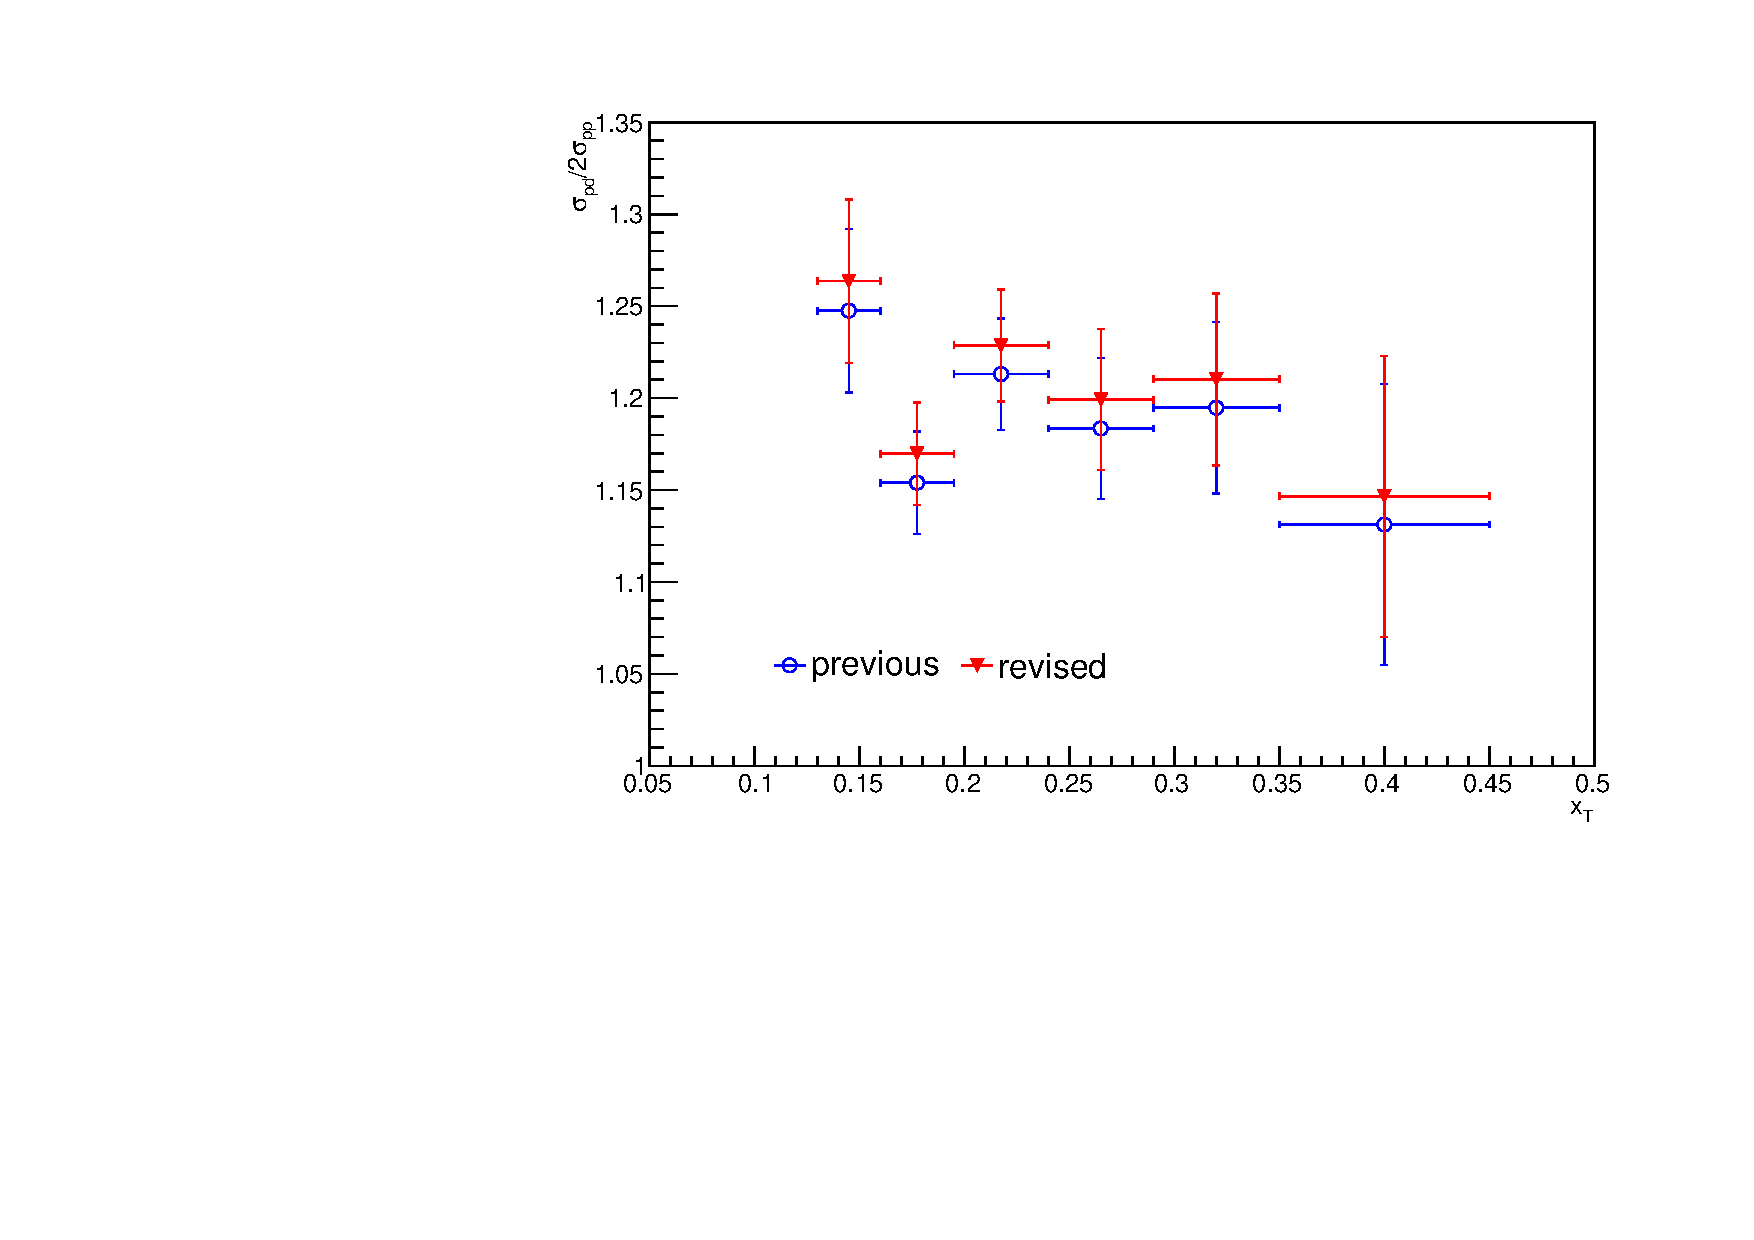
\includegraphics[width=0.6\linewidth]{DY-csr/Compare_targetCorr}
	\caption{The effect of the updated target contamination correction on the Drell-Y.an
		cross section. The extracted cross section ratio using the revised target contamination
		is shown as red sold triangle, and the previous published version is shown as blue open
		circle. The overall effect is a roughly \SI{2}{\percent} shift in the ratio. }
	\label{fig:contaimination_CSR}
\end{figure}



\subsubsection{Choice of fit function in intensity extrapolation}
To understand the systematic uncertainties in the intensity extrapolation method due to the
choice of fit function, the following functions are used.
\begin{align}
	R_i\left(I\right) & = p_{0i} + p_{1} I + p_{2} I^2 \quad\text{(FIT 1)}                                                     \\
	R_i\left(I\right) & = p_{0i} + \left[p_{10} + p_{11}x_i\right] I + \left[p_{20} + p_{21}x_i\right]I^2 \quad \text{(FIT 2)}
\end{align}
The fit to data using the two fits are shown in \cref{fig:run2-3_FIT1_xT,fig:run2-3_FIT2_xT}
and $\chi^2$ for the fits are tabulated in \cref{tab:chi_run23}.
And the fit for other variables are listed in \cref{M-a_ch:extrapolation}.
\begin{figure}
	\centering
	\caption{Fit to the flask subtracted yield ratio with FIT1 for $x_T$ for run 2-3.}
	\label{fig:run2-3_FIT1_xT}
	\begin{subfigure}{0.45\linewidth}
		\includegraphics[width=\linewidth]{extrapolation/run2-3/xT/FIT1/hist_fitted_xT_tInt_0}
	\end{subfigure}
	\begin{subfigure}{0.45\linewidth}
		\includegraphics[width=\linewidth]{extrapolation/run2-3/xT/FIT1/hist_fitted_xT_tInt_1}
	\end{subfigure}
	\begin{subfigure}{0.45\linewidth}
		\includegraphics[width=\linewidth]{extrapolation/run2-3/xT/FIT1/hist_fitted_xT_tInt_2}
	\end{subfigure}
	\begin{subfigure}{0.45\linewidth}
		\includegraphics[width=\linewidth]{extrapolation/run2-3/xT/FIT1/hist_fitted_xT_tInt_3}
	\end{subfigure}
	\begin{subfigure}{0.45\linewidth}
		\includegraphics[width=\linewidth]{extrapolation/run2-3/xT/FIT1/hist_fitted_xT_tInt_4}
	\end{subfigure}
	\begin{subfigure}{0.45\linewidth}
		\includegraphics[width=\linewidth]{extrapolation/run2-3/xT/FIT1/hist_fitted_xT_tInt_5}
	\end{subfigure}
\end{figure}

\begin{figure}
	\centering
	\caption{Fit to the flask subtracted yield ratio with FIT2 for $x_T$ for run 2-3.}
	\label{fig:run2-3_FIT2_xT}
	\begin{subfigure}{0.45\linewidth}
		\includegraphics[width=\linewidth]{extrapolation/run2-3/xT/FIT2/hist_fitted_xT_tInt_0}
	\end{subfigure}
	\begin{subfigure}{0.45\linewidth}
		\includegraphics[width=\linewidth]{extrapolation/run2-3/xT/FIT2/hist_fitted_xT_tInt_1}
	\end{subfigure}
	\begin{subfigure}{0.45\linewidth}
		\includegraphics[width=\linewidth]{extrapolation/run2-3/xT/FIT2/hist_fitted_xT_tInt_2}
	\end{subfigure}
	\begin{subfigure}{0.45\linewidth}
		\includegraphics[width=\linewidth]{extrapolation/run2-3/xT/FIT2/hist_fitted_xT_tInt_3}
	\end{subfigure}
	\begin{subfigure}{0.45\linewidth}
		\includegraphics[width=\linewidth]{extrapolation/run2-3/xT/FIT2/hist_fitted_xT_tInt_4}
	\end{subfigure}
	\begin{subfigure}{0.45\linewidth}
		\includegraphics[width=\linewidth]{extrapolation/run2-3/xT/FIT2/hist_fitted_xT_tInt_5}
	\end{subfigure}
\end{figure}



\Cref{fig:CSR_Run2-3} shows the extracted cross section ratio as a function of $x_T$, $x_B$ and $x_F$.
While the two fit functions produce similar results for $x_T$, the differences are slightly larger in
the other variables.

\begin{figure}[h!]
	\centering
	\begin{subfigure}{0.6\linewidth}
		\includegraphics*[width=\linewidth]{DY-csr/run23_xT}
	\end{subfigure}\\
	\begin{subfigure}{0.45\linewidth}
		\includegraphics*[width=\linewidth]{DY-csr/run23_xB}
	\end{subfigure}
	\begin{subfigure}{0.45\linewidth}
		\includegraphics*[width=\linewidth]{DY-csr/run23_xF}
	\end{subfigure}
	\caption{Comparison of the extracted Drell-Yan cross section ratio as a function of $x_T$(top),
		$x_B$(left) and $x_F$(right) using the different methods from the Run 2-3
		data.}
	\label{fig:CSR_Run2-3}
\end{figure}

\begin{table}[h!]
	\centering
	\caption{The reduced $\chi^2$ for the different fits used in the intensity extrapolation method for Run 2-3. }
	\label{tab:chi_run23}
	\begin{tabular}{|l|lll|}
\hline
 & \multicolumn{3}{c|}{$\chi^2/NDF$} \\ \cline{2-4} 
      & \multicolumn{1}{c|}{$x_T$}          & \multicolumn{1}{c|}{$x_B$}          & \multicolumn{1}{c|}{$x_F$} \\ \hline
FIT 1 & \multicolumn{1}{l|}{$40.1167 / 40$} & \multicolumn{1}{l|}{$71.3796 / 47$} & $68.0593 / 47$             \\ \hline
FIT 2 & \multicolumn{1}{l|}{$40.008 / 38$}  & \multicolumn{1}{l|}{$61.8549 / 45$} & $64.1524 / 45$             \\ \hline
\end{tabular}

\end{table}


\subsubsection{Comparison of massfit and extrapolation}
\Cref{fig:massfit_integrated_run23} shows the fit to the mass distributions for Run 2-3 data, and the
data is very well described by the fitting procedure.
\begin{figure}[h!]
	\begin{subfigure}{0.45\linewidth}
		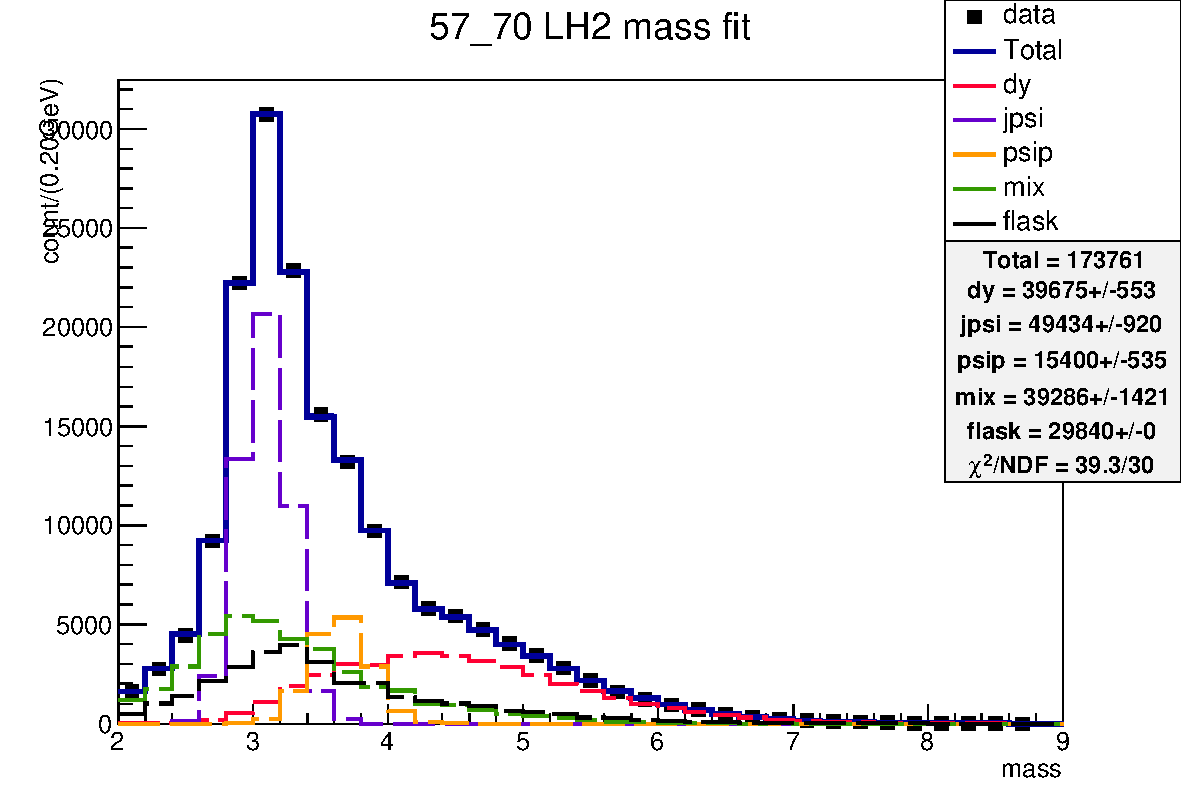
\includegraphics[width=\linewidth]{massfit/run2-3/57_70_LH2}
	\end{subfigure}
	\begin{subfigure}{0.45\linewidth}
		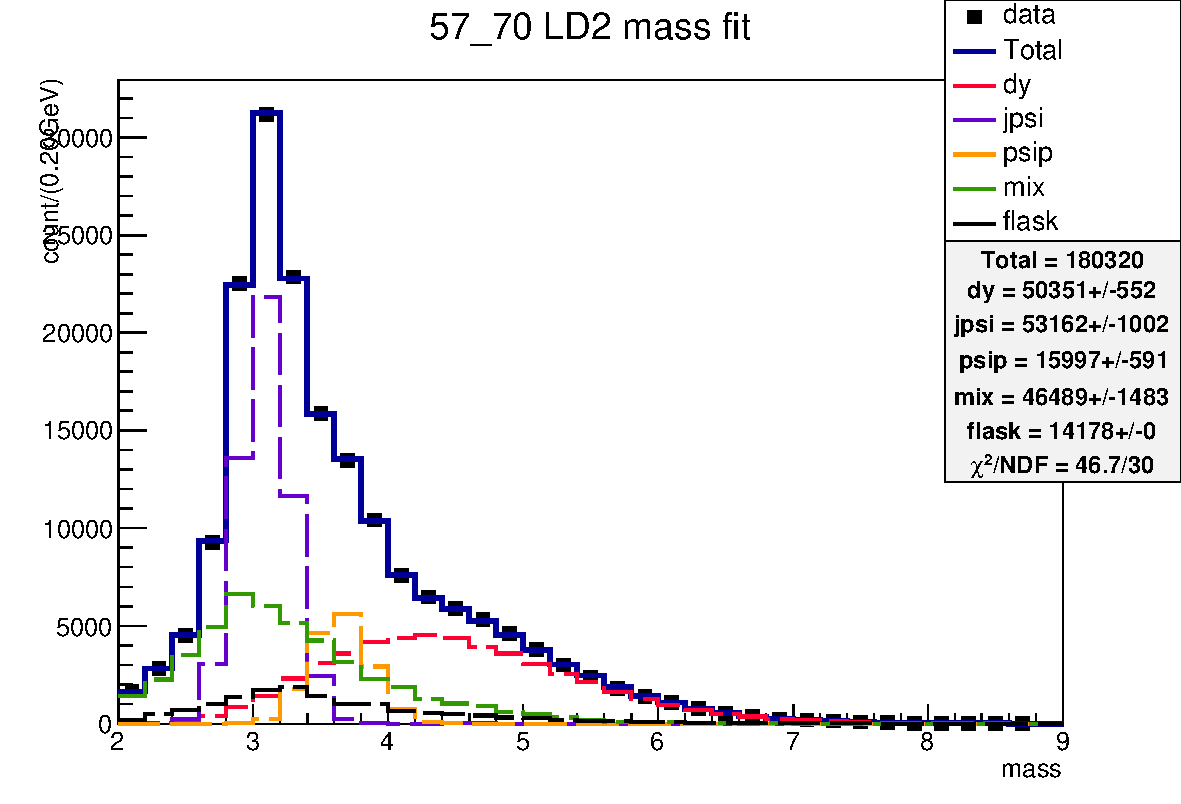
\includegraphics[width=\linewidth]{massfit/run2-3/57_70_LD2}
	\end{subfigure}
	\caption{The mass spectrum for \ce{LH_2}(left) and \ce{LD_2}(right) targets data for Run 2-3}
	\label{fig:massfit_integrated_run23}
\end{figure}

With the yield for different process obtained from the mass fits, the cross section ratios can be calculated
and are also shown in \cref{fig:CSR_Run2-3}.
As reported in Ref.~\cite{dove2023} the Drell-Yan cross section ratio as a function of $x_T$ extracted from
the two methods are in very good agreement.

However, the comparison in other variables, such as $x_B$ and $x_F$ are complicated by the large
systematical uncertainties originated from the fit function used in the intensity extrapolation.
\Cref{fig:CSR_Run2-3} shows the extracted ratios as a function of $x_B$ and $x_F$ using different methods.
While the massfit results agree with the extrapolation result if FIT 1 is used, the
extrapolation results using FIT 2 are different from the other two.

\FloatBarrier

\subsection{Results from Run 5-6 data}
\Cref{fig:massfit_integrated_run56} shows the fit to the mass distributions for Run 5-6 data,
and the data is very well described by the fitting procedure.
\begin{figure}[h!]
	\begin{subfigure}{0.45\linewidth}
		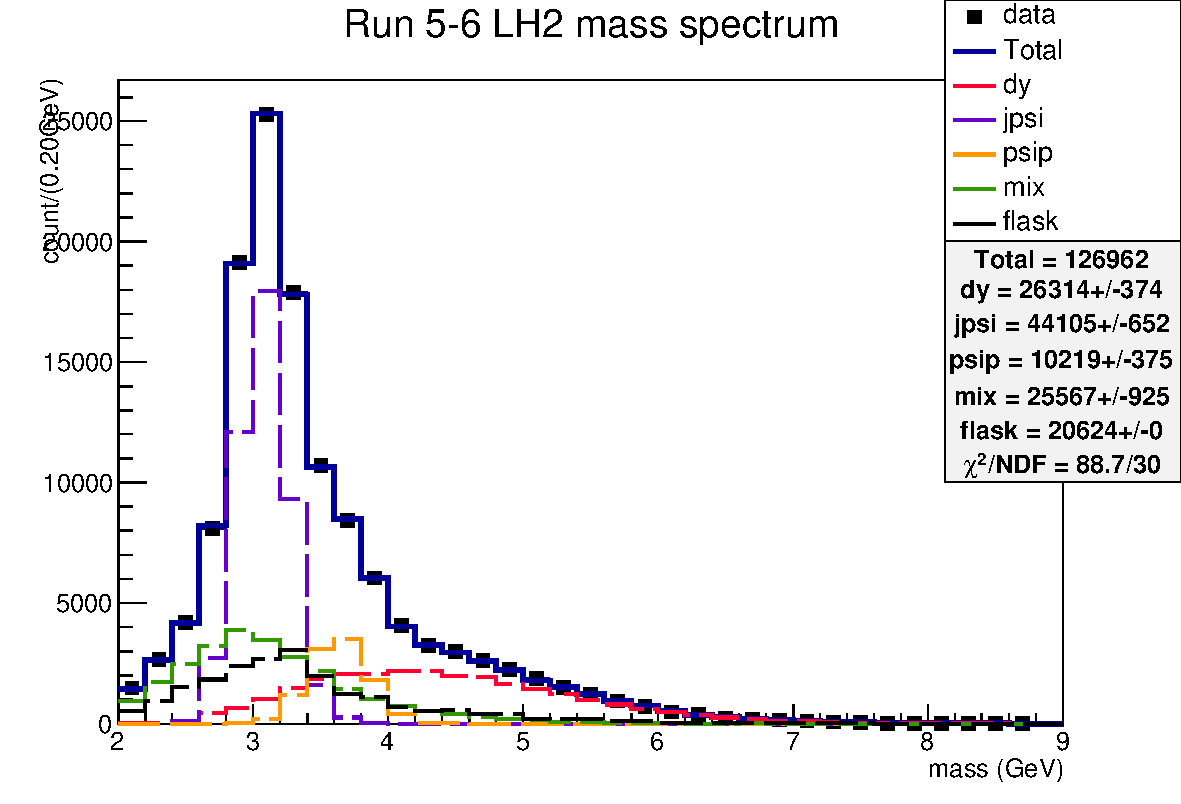
\includegraphics[width=\linewidth]{massfit/run5-6/5_6_LH2}
	\end{subfigure}
	\begin{subfigure}{0.45\linewidth}
		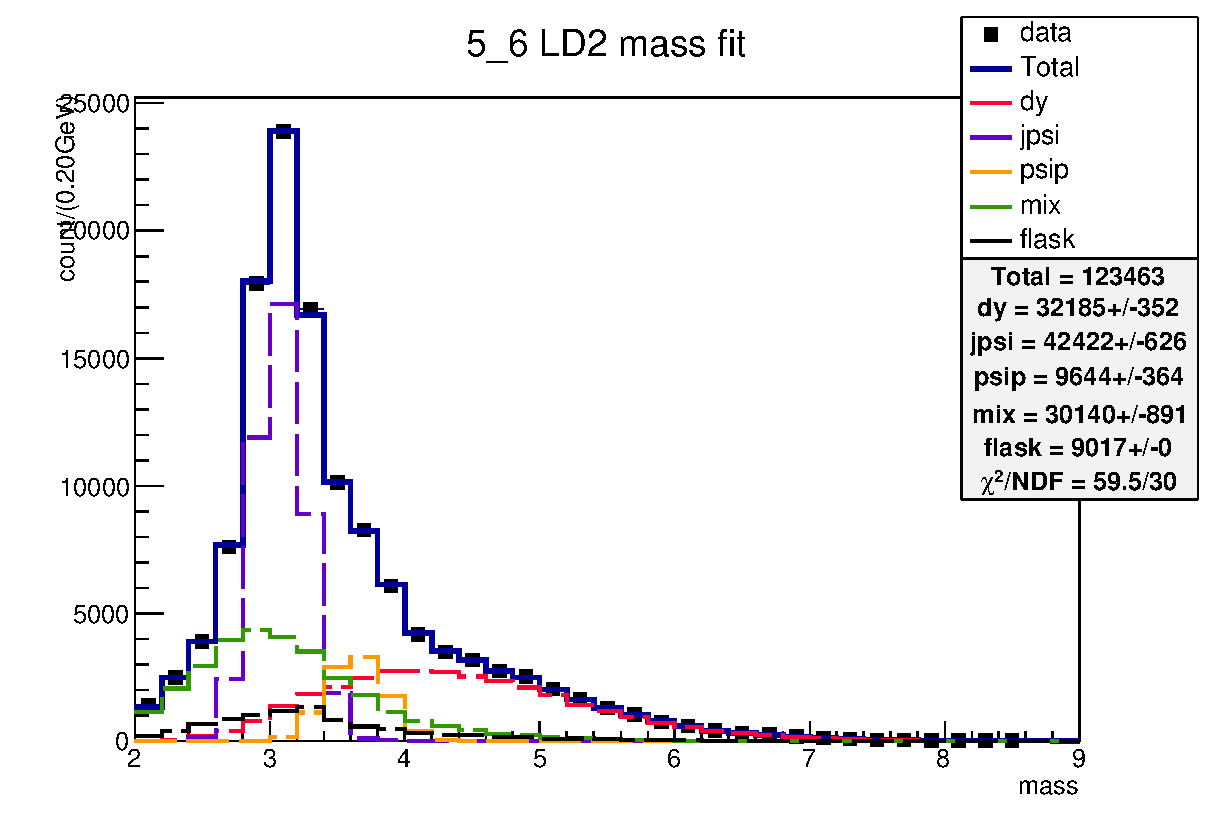
\includegraphics[width=\linewidth]{massfit/run5-6/5_6_LD2}
	\end{subfigure}
	\caption{The mass spectrum for \ce{LH_2}(left) and \ce{LD_2}(right) targets data for Run 5-6}
	\label{fig:massfit_integrated_run56}
\end{figure}
The Drell-Yan yield for $p+p$ and $p+d$ can then be extracted and the cross section ratio
is shown in \cref{fig:CSR_Run5-6}.

To extract the cross section ratio using the intensity extrapolation method, yield ratio
calculated as function of $x_T$ and intensity and the fits are shown in \cref{fig:run5-6_FIT1_xT}
(FIT 1) and \cref{fig:run5-6_FIT2_xT} (FIT 2), with the fits for other variables listed in
\cref{M-a_ch:extrapolation}. And the reduced $\chi^2$ is tabulated in \cref{tab:chi_run56}.
\begin{figure}
\begin{subfigure}{0.45\linewidth}
\includegraphics{width=\linewidth}{extrapolation/run5-6/xT/FIT1/hist_fitted_xT_tInt_0}
\end{subfigure}
\begin{subfigure}{0.45\linewidth}
\includegraphics{width=\linewidth}{extrapolation/run5-6/xT/FIT1/hist_fitted_xT_tInt_1}
\end{subfigure}
\begin{subfigure}{0.45\linewidth}
\includegraphics{width=\linewidth}{extrapolation/run5-6/xT/FIT1/hist_fitted_xT_tInt_2}
\end{subfigure}
\begin{subfigure}{0.45\linewidth}
\includegraphics{width=\linewidth}{extrapolation/run5-6/xT/FIT1/hist_fitted_xT_tInt_3}
\end{subfigure}
\begin{subfigure}{0.45\linewidth}
\includegraphics{width=\linewidth}{extrapolation/run5-6/xT/FIT1/hist_fitted_xT_tInt_4}
\end{subfigure}
\begin{subfigure}{0.45\linewidth}
\includegraphics{width=\linewidth}{extrapolation/run5-6/xT/FIT1/hist_fitted_xT_tInt_5}
\end{subfigure}
\end{figure}

\begin{figure}
	\centering
	\caption{Fit to the flask subtracted yield ratio with FIT2 for $x_T$ for run 5-6.}
	\label{fig:run5-6_FIT2_xT}
	\begin{subfigure}{0.45\linewidth}
		\includegraphics[width=\linewidth]{extrapolation/run5-6/xT/FIT2/hist_fitted_xT_tInt_0}
	\end{subfigure}
	\begin{subfigure}{0.45\linewidth}
		\includegraphics[width=\linewidth]{extrapolation/run5-6/xT/FIT2/hist_fitted_xT_tInt_1}
	\end{subfigure}
	\begin{subfigure}{0.45\linewidth}
		\includegraphics[width=\linewidth]{extrapolation/run5-6/xT/FIT2/hist_fitted_xT_tInt_2}
	\end{subfigure}
	\begin{subfigure}{0.45\linewidth}
		\includegraphics[width=\linewidth]{extrapolation/run5-6/xT/FIT2/hist_fitted_xT_tInt_3}
	\end{subfigure}
	\begin{subfigure}{0.45\linewidth}
		\includegraphics[width=\linewidth]{extrapolation/run5-6/xT/FIT2/hist_fitted_xT_tInt_4}
	\end{subfigure}
	\begin{subfigure}{0.45\linewidth}
		\includegraphics[width=\linewidth]{extrapolation/run5-6/xT/FIT2/hist_fitted_xT_tInt_5}
	\end{subfigure}
\end{figure}

From the fits, the cross section ratio can be extracted.

\pdfmargincomment{run 5-6 compared with 2-3 and full data set, only show massfit results?}
\Cref{fig:CSR_Run5-6} shows the extracted cross section ratio as a function from the
second half of our data using various methods. While the different fit functions used in the
intensity extrapolation produce very similar results, the massfit result is significantly larger
than the intensity extrapolation results. This difference is included in the systematic uncertainties
for the final Drell-Yan cross section ratio from Run 5-6.
\begin{figure}[h!]
	\centering
	\begin{subfigure}{0.6\linewidth}
		\includegraphics*[width=\linewidth]{DY-csr/run56_xT}
	\end{subfigure}
	\begin{subfigure}{0.45\linewidth}
		\includegraphics*[width=\linewidth]{DY-csr/run56_xB}
	\end{subfigure}
	\begin{subfigure}{0.45\linewidth}
		\includegraphics*[width=\linewidth]{DY-csr/run56_xF}
	\end{subfigure}
	\caption{Comparison of the extracted Drell-Yan cross section ratio as a function of $x_T$(top),  $x_B$(left)
		and $x_F$(right) from the Run 5-6 data using the massfit and intensity extrapolation method.}
	\label{fig:CSR_Run5-6}
\end{figure}
\begin{table}
	\centering
	\caption{The reduced $\chi^2$ for the different fits used in the intensity extrapolation method for Run 5-6. }
	\label{tab:chi_run56}
	\begin{tabular}{|l|lll|}
\hline
 & \multicolumn{3}{c|}{$\chi^2/NDF$} \\ \cline{2-4} 
      & \multicolumn{1}{c|}{$x_T$}          & \multicolumn{1}{c|}{$x_B$}          & \multicolumn{1}{c|}{$x_F$} \\ \hline
FIT 1 & \multicolumn{1}{l|}{$24.3236 / 28$} & \multicolumn{1}{l|}{$41.6412 / 33$} & $28.1757 / 33$             \\ \hline
FIT 2 & \multicolumn{1}{l|}{$23.2091 / 26$}  & \multicolumn{1}{l|}{$40.3455 / 31$} & $25.7949 / 31$             \\ \hline
\end{tabular}

\end{table}

\subsubsection{Potential cause of difference between massfit and intensity extrapolation}
During the second half of the data taking, the variation in the instantaneous beam
intensity was reduced as compared to run 2-3. This is partly due to the improvement
in beam quality and partly due to the tightening of the beam inhibit thresholds.

The massfit and intensity extrapolation methods made different assumption on the intensity
and rate dependence. With less high intensity data, there are less constraints on the
intensity dependence, causing the two method to disagree.

\pdfcomment{Intensity range cannot explain the discrepancy }
\Cref{fig:CSR_combined} shows the final results from the two datasets. The two datasets
are consistent with each other, partly due to the large systematic uncertainties in the
Run 5-6 results, which is dominated by the differences between the massfit and intensity
extrapolation methods.
\begin{figure}
	\centering
	\begin{subfigure}{0.6\linewidth}
		\includegraphics*[width=\linewidth]{DY-csr/combined_xT}
	\end{subfigure}
	\begin{subfigure}{0.45\linewidth}
		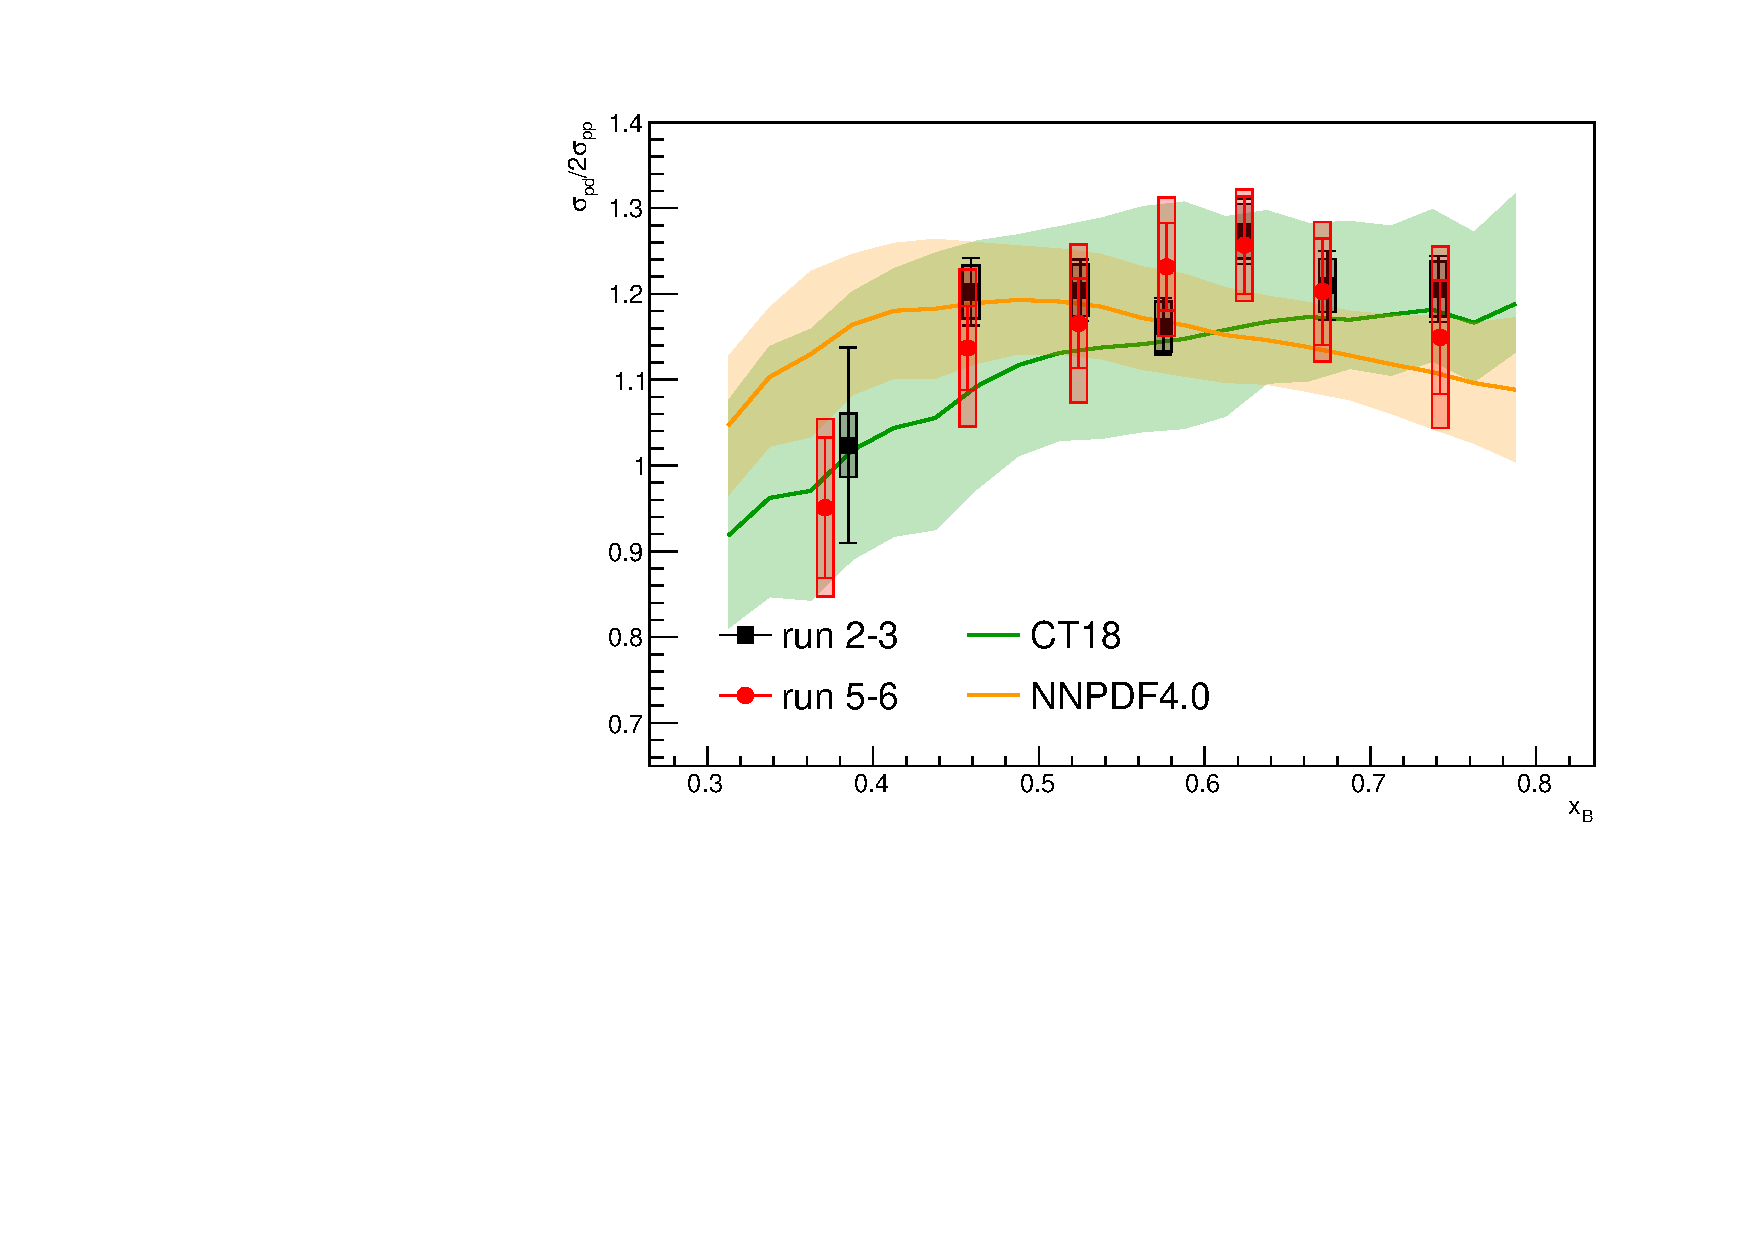
\includegraphics[width=\linewidth]{DY-csr/combined_xB}
	\end{subfigure}
	\begin{subfigure}{0.45\linewidth}
		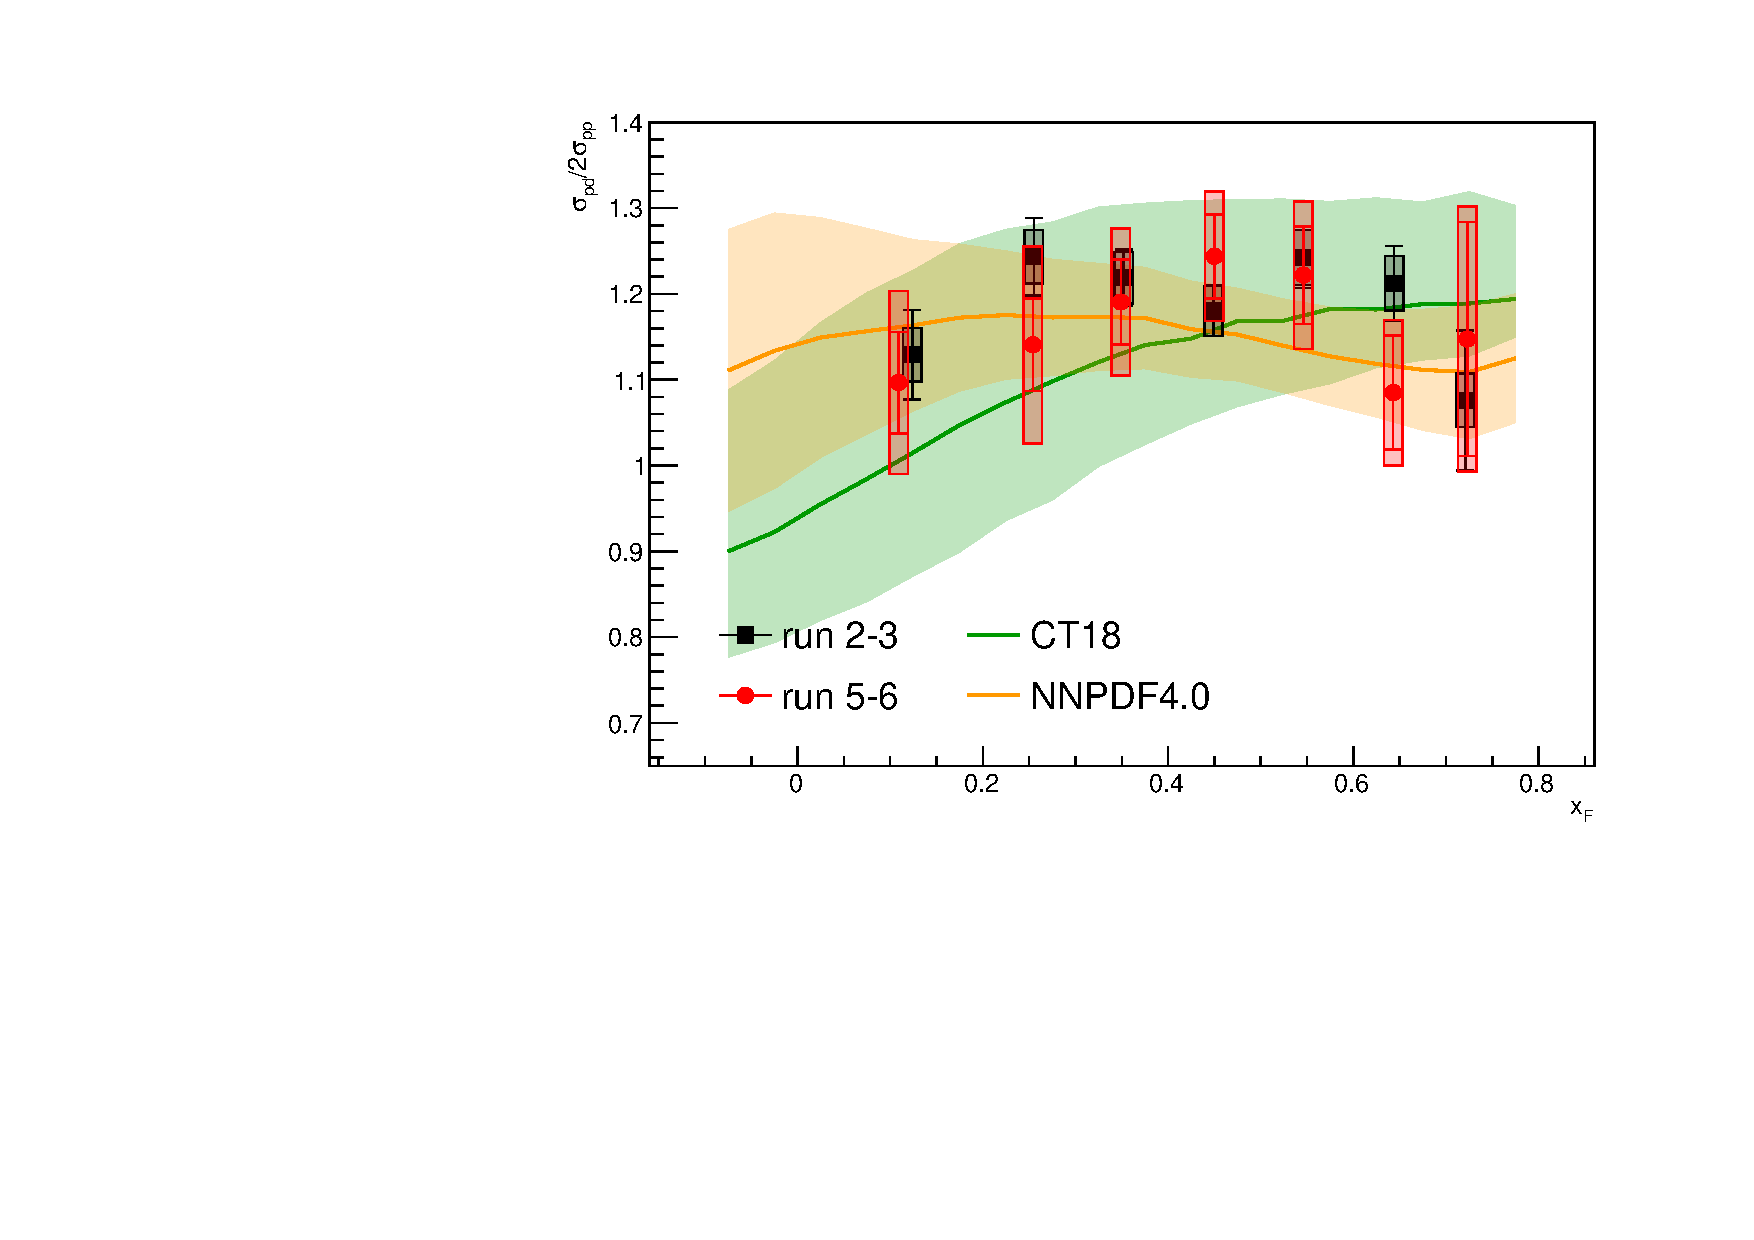
\includegraphics[width=\linewidth]{DY-csr/combined_xF}
	\end{subfigure}
	\caption{Comparison of the extracted Drell-Yan cross section ratio as a function of $x_T$(top),  $x_B$(left)
		and $x_F$(right) from the two datasets.}
	\label{fig:CSR_combined}
\end{figure}


\subsection{Comparison with global PDF analysis}
\pdfmargincomment{modified to impact of SeaQuest result?}
The published $\sigma_{pd}/2\sigma_{pp}$ ratio result has been included in various recent global
PDF analysis, including Ref.~\cite{cocuzza2021,guzzi2022,accardi2023,alekhin2023}.
In particular, \cref{fig:CSR_Run2-3} shows the calculation using CT18 (without the SeaQuest data)
and NNPDF 4.0 (including the SeaQuest data). The shift in the cross section ratio is primarily
coming from the inclusion of the SeaQuest data. Unlike the previous E866 result, the SeaQuest data
strongly suggests the $\bar{d}/\bar{u}$ ratio would remain greater than one for $x<0.4$, which is
consistent with prediction from various models, including meson cloud and statistical model.

The importance of the SeaQuest data can be seen in the NNPDF 4.0, where at large $x_T$,
uncertainties bands is consistent with the uncertainties of our measurements, as the SeaQuest
results is the only available data sensitive to the light sea-quark asymmetry at large $x$.
\FloatBarrier

\section{Charmonium Cross Section}

\subsection{Massfit results}
The massfits in all $x_F$ bins are shown in \cref{fig:massfit_57-70_xF,fig:massfit_5-6_xF},
and the fits in the $P_T$ bins are shown in \cref{fig:massfit_57-70_pT,fig:massfit_5-6_pT}.
The two datasets are analyzed separately. The data in each bin is very well described by the fitting procedure
and the $J/\psi$ and $\psi'$ yields can be extracted from the fits directly.
\pdfmargincomment{undate massfit plots!!!}
\begin{figure}[h]
	\centering
	\begin{subfigure}{0.4\linewidth}
		\includegraphics[width=0.9\linewidth]{massfit/run2-3/LH2/xF/LH2_xFbin0}
	\end{subfigure}
	\begin{subfigure}{0.4\linewidth}
		\includegraphics[width=0.9\linewidth]{massfit/run2-3/LD2/xF/LD2_xFbin0}
	\end{subfigure}\\
	\begin{subfigure}{0.4\linewidth}
		\includegraphics[width=0.9\linewidth]{massfit/run2-3/LH2/xF/LH2_xFbin1}
	\end{subfigure}
	\begin{subfigure}{0.4\linewidth}
		\includegraphics[width=0.9\linewidth]{massfit/run2-3/LD2/xF/LD2_xFbin1}
	\end{subfigure}\\
	\begin{subfigure}{0.4\linewidth}
		\includegraphics[width=0.9\linewidth]{massfit/run2-3/LH2/xF/LH2_xFbin2}
	\end{subfigure}
	\begin{subfigure}{0.4\linewidth}
		\includegraphics[width=0.9\linewidth]{massfit/run2-3/LD2/xF/LD2_xFbin2}
	\end{subfigure}\\
	\begin{subfigure}{0.4\linewidth}
		\includegraphics[width=0.9\linewidth]{massfit/run2-3/LH2/xF/LH2_xFbin3}
	\end{subfigure}
	\begin{subfigure}{0.4\linewidth}
		\includegraphics[width=0.9\linewidth]{massfit/run2-3/LD2/xF/LD2_xFbin3}
	\end{subfigure}\\
	\begin{subfigure}{0.4\linewidth}
		\includegraphics[width=0.9\linewidth]{massfit/run2-3/LH2/xF/LH2_xFbin4}
	\end{subfigure}
	\begin{subfigure}{0.4\linewidth}
		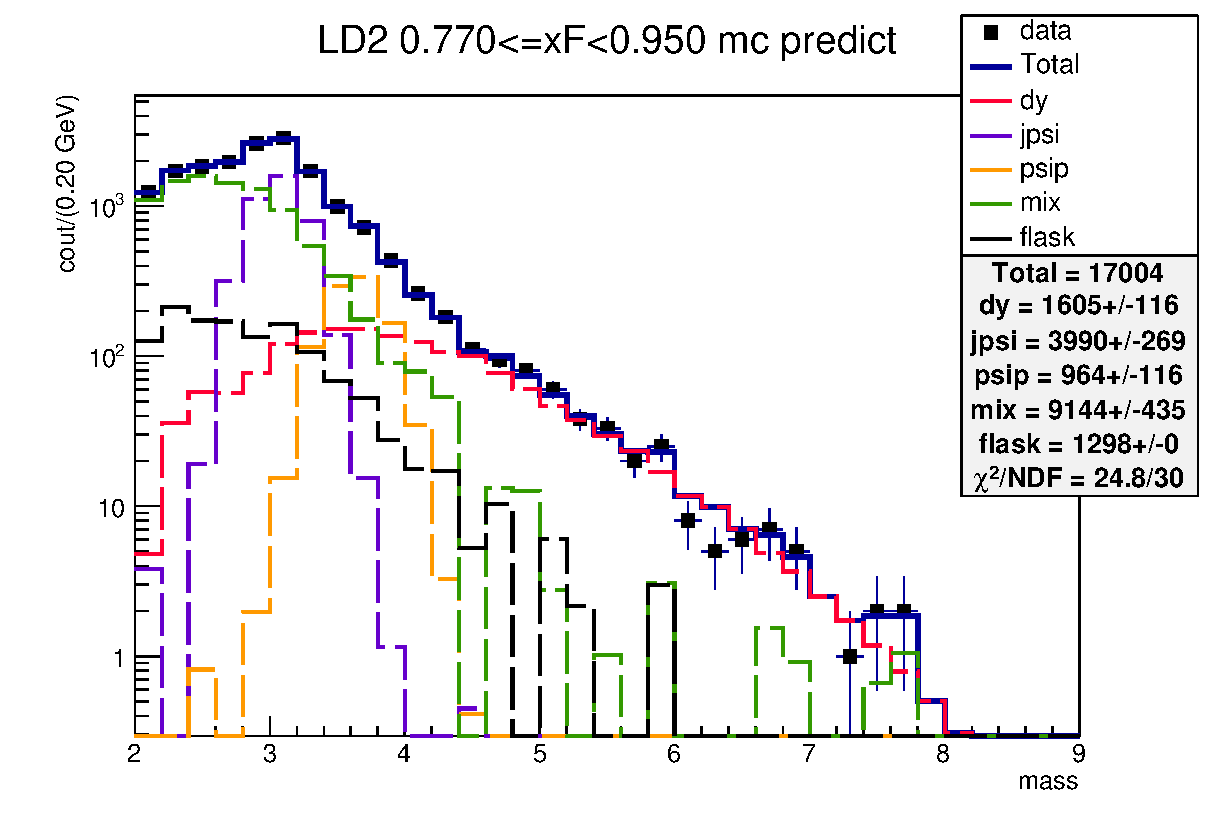
\includegraphics[width=0.9\linewidth]{massfit/run2-3/LD2/xF/LD2_xFbin4}
	\end{subfigure}
	\caption{Mass fit for run 2-3 data in each $x_F$ bin for both \ce{LH_2}(left) and \ce{LD_2}(right) targets. }
	\label{fig:massfit_57-70_xF}
\end{figure}

\begin{figure}[h]
	\centering
	\begin{subfigure}{0.4\linewidth}
		\includegraphics[width=0.9\linewidth]{massfit/run5-6/LH2/xF/LH2_xFbin0}
	\end{subfigure}
	\begin{subfigure}{0.4\linewidth}
		\includegraphics[width=0.9\linewidth]{massfit/run5-6/LD2/xF/LD2_xFbin0}
	\end{subfigure}\\
	\begin{subfigure}{0.4\linewidth}
		\includegraphics[width=0.9\linewidth]{massfit/run5-6/LH2/xF/LH2_xFbin1}
	\end{subfigure}
	\begin{subfigure}{0.4\linewidth}
		\includegraphics[width=0.9\linewidth]{massfit/run5-6/LD2/xF/LD2_xFbin1}
	\end{subfigure}\\
	\begin{subfigure}{0.4\linewidth}
		\includegraphics[width=0.9\linewidth]{massfit/run5-6/LH2/xF/LH2_xFbin2}
	\end{subfigure}
	\begin{subfigure}{0.4\linewidth}
		\includegraphics[width=0.9\linewidth]{massfit/run5-6/LD2/xF/LD2_xFbin2}
	\end{subfigure}\\
	\begin{subfigure}{0.4\linewidth}
		\includegraphics[width=0.9\linewidth]{massfit/run5-6/LH2/xF/LH2_xFbin3}
	\end{subfigure}
	\begin{subfigure}{0.4\linewidth}
		\includegraphics[width=0.9\linewidth]{massfit/run5-6/LD2/xF/LD2_xFbin3}
	\end{subfigure}\\
	\begin{subfigure}{0.4\linewidth}
		\includegraphics[width=0.9\linewidth]{massfit/run5-6/LH2/xF/LH2_xFbin4}
	\end{subfigure}
	\begin{subfigure}{0.4\linewidth}
		\includegraphics[width=0.9\linewidth]{massfit/run5-6/LD2/xF/LD2_xFbin4}
	\end{subfigure}
	\caption{Mass fit for run 5-6 data in each $x_F$ bin for both \ce{LH_2}(left) and \ce{LD_2}(right) targets. }
	\label{fig:massfit_5-6_xF}
\end{figure}

\begin{figure}[h]
	\centering
	\begin{subfigure}{0.4\linewidth}
		\includegraphics[width=0.9\linewidth]{massfit/run2-3/LH2/pT/LH2_pTbin0}
	\end{subfigure}
	\begin{subfigure}{0.4\linewidth}
		\includegraphics[width=0.9\linewidth]{massfit/run2-3/LD2/pT/LD2_pTbin0}
	\end{subfigure}\\
	\begin{subfigure}{0.4\linewidth}
		\includegraphics[width=0.9\linewidth]{massfit/run2-3/LH2/pT/LH2_pTbin1}
	\end{subfigure}
	\begin{subfigure}{0.4\linewidth}
		\includegraphics[width=0.9\linewidth]{massfit/run2-3/LD2/pT/LD2_pTbin1}
	\end{subfigure}\\
	\begin{subfigure}{0.4\linewidth}
		\includegraphics[width=0.9\linewidth]{massfit/run2-3/LH2/pT/LH2_pTbin2}
	\end{subfigure}
	\begin{subfigure}{0.4\linewidth}
		\includegraphics[width=0.9\linewidth]{massfit/run2-3/LD2/pT/LD2_pTbin2}
	\end{subfigure}\\
	\begin{subfigure}{0.4\linewidth}
		\includegraphics[width=0.9\linewidth]{massfit/run2-3/LH2/pT/LH2_pTbin3}
	\end{subfigure}
	\begin{subfigure}{0.4\linewidth}
		\includegraphics[width=0.9\linewidth]{massfit/run2-3/LD2/pT/LD2_pTbin3}
	\end{subfigure}\\
	\begin{subfigure}{0.4\linewidth}
		\includegraphics[width=0.9\linewidth]{massfit/run2-3/LH2/pT/LH2_pTbin4}
	\end{subfigure}
	\begin{subfigure}{0.4\linewidth}
		\includegraphics[width=0.9\linewidth]{massfit/run2-3/LD2/pT/LD2_pTbin4}
	\end{subfigure}
	\caption{Mass fit for run 2-3 data in each $P_T$ bin for both \ce{LH_2}(left) and \ce{LD_2}(right) targets. }
	\label{fig:massfit_57-70_pT}
\end{figure}

\begin{figure}[h]
	\centering
	\begin{subfigure}{0.4\linewidth}
		\includegraphics[width=0.9\linewidth]{massfit/run5-6/LH2/pT/LH2_pTbin0}
	\end{subfigure}
	\begin{subfigure}{0.4\linewidth}
		\includegraphics[width=0.9\linewidth]{massfit/run5-6/LD2/pT/LD2_pTbin0}
	\end{subfigure}\\
	\begin{subfigure}{0.4\linewidth}
		\includegraphics[width=0.9\linewidth]{massfit/run5-6/LH2/pT/LH2_pTbin1}
	\end{subfigure}
	\begin{subfigure}{0.4\linewidth}
		\includegraphics[width=0.9\linewidth]{massfit/run5-6/LD2/pT/LD2_pTbin1}
	\end{subfigure}\\
	\begin{subfigure}{0.4\linewidth}
		\includegraphics[width=0.9\linewidth]{massfit/run5-6/LH2/pT/LH2_pTbin2}
	\end{subfigure}
	\begin{subfigure}{0.4\linewidth}
		\includegraphics[width=0.9\linewidth]{massfit/run5-6/LD2/pT/LD2_pTbin2}
	\end{subfigure}\\
	\begin{subfigure}{0.4\linewidth}
		\includegraphics[width=0.9\linewidth]{massfit/run5-6/LH2/pT/LH2_pTbin3}
	\end{subfigure}
	\begin{subfigure}{0.4\linewidth}
		\includegraphics[width=0.9\linewidth]{massfit/run5-6/LD2/pT/LD2_pTbin3}
	\end{subfigure}\\
	\begin{subfigure}{0.4\linewidth}
		\includegraphics[width=0.9\linewidth]{massfit/run5-6/LH2/pT/LH2_pTbin4}
	\end{subfigure}
	\begin{subfigure}{0.4\linewidth}
		\includegraphics[width=0.9\linewidth]{massfit/run5-6/LD2/pT/LD2_pTbin4}
	\end{subfigure}
	\caption{Mass fit for run 5-6 data in each $P_T$ bin for both \ce{LH_2}(left) and \ce{LD_2}(right) targets. }
	\label{fig:massfit_5-6_pT}
\end{figure}


\FloatBarrier

\subsection{\texorpdfstring{$x_F$}{x\_F} distributions}
With the yields extracted, the cross section can be calculated.
\begin{figure}[h!]
	\centering
	\begin{subfigure}{0.45\linewidth}
		\includegraphics[width=\linewidth]{cs/xF/combine_xF_LH2_5-6_5770_psip}
	\end{subfigure}
	\centering
	\begin{subfigure}{0.45\linewidth}
		\includegraphics[width=\linewidth]{cs/xF/combine_xF_LD2_5-6_5770_psip}
	\end{subfigure}
	\\
	\begin{subfigure}{0.45\linewidth}
		\includegraphics[width=\linewidth]{cs/xF/ratio_xF_LH2_5-6_5770}
	\end{subfigure}
	\begin{subfigure}{0.45\linewidth}
		\includegraphics[width=\linewidth]{cs/xF/ratio_xF_LD2_5-6_5770}
	\end{subfigure}
	\caption{The extracted $J/\psi$ and $\psi'$ cross section (top) and $\sigma_{\psi'}/\sigma_{J/\psi}$
		ratio (bottom) as a function of $x_F$ for $p+p$(left) and $p+d$(right) from the two datasets,
		and compared with the NRQCD predictions}
	\label{fig:cs_xF}
\end{figure}
The extracted cross section for $J/\psi$ and $\psi'$ from the two datasets are shown in \cref{fig:cs_xF}, and are
tabulated in \cref{tab:xF_57-70_LH2,tab:xF_57-70_LD2,tab:xF_5-6_LH2,tab:xF_5-6_LD2}.
The results from the two datasets are in very good agreement.

\begin{table}[h!]
	\centering
	\caption{Cross section as a function of $x_F$ (in \unit{\nano\barn\per nucleon}) and the
		$\sigma_{\psi'}/\sigma_{J/\psi}$ ratio for $p+p$ extracted from run 2-3, with their statistical
		and systematic uncertainties and the average $x_F$ in each bin.}
	\begin{tabular}{cc|cc|c}
\hline
\multicolumn{2}{c|}{$J/\psi$} &
  \multicolumn{2}{c|}{$\psi^{\prime}$} &
  \multirow{2}{*}{$\sigma_{\psi^\prime}/\sigma_{J/\psi}$} \\ \cline{1-4}
$\expval{x_F}_{J/\psi}$ &
  $\eval{d\sigma/dx_F}_{J/\psi}$ &
  $\expval{x_F}_{\psi^\prime}$ &
  $\eval{d\sigma/dx_F}_{\psi^\prime}$ &
   \\ \hline
\multicolumn{1}{c|}{0.527} &
  $6.609\pm0.365\pm1.664$ &
  \multicolumn{1}{c|}{0.509} &
  $1.8458\pm0.1410\pm0.2685$ &
  $0.279\pm0.026\pm0.082$ \\
\multicolumn{1}{c|}{0.625} &
  $3.057\pm0.183\pm0.486$ &
  \multicolumn{1}{c|}{0.624} &
  $0.9631\pm0.0953\pm0.1537$ &
  $0.315\pm0.036\pm0.019$ \\
\multicolumn{1}{c|}{0.672} &
  $1.996\pm0.111\pm0.259$ &
  \multicolumn{1}{c|}{0.672} &
  $0.6165\pm0.0615\pm0.0651$ &
  $0.309\pm0.035\pm0.024$ \\
\multicolumn{1}{c|}{0.732} &
  $1.041\pm0.050\pm0.166$ &
  \multicolumn{1}{c|}{0.733} &
  $0.3480\pm0.0357\pm0.0605$ &
  $0.334\pm0.038\pm0.036$ \\
\multicolumn{1}{c|}{0.814} &
  $0.210\pm0.013\pm0.043$ &
  \multicolumn{1}{c|}{0.821} &
  $0.0754\pm0.0110\pm0.0076$ &
  $0.358\pm0.057\pm0.053$ \\ \hline
\end{tabular}

	\label{tab:xF_57-70_LH2}
\end{table}
\begin{table}[h!]
	\centering
	\caption{Cross section as a function of $x_F$ (in \unit{\nano\barn\per nucleon}) and the
		$\sigma_{\psi'}/\sigma_{J/\psi}$ ratio for $p+d$ extracted from run 2-3, with their statistical
		and systematic uncertainties and the average $x_F$ in each bin.}
	\begin{tabular}{cc|cc|c}
\hline
\multicolumn{2}{c|}{$J/\psi$} &
  \multicolumn{2}{c|}{$\psi^{\prime}$} &
  \multirow{2}{*}{$\sigma_{\psi^\prime}/\sigma_{J/\psi}$} \\ \cline{1-4}
$\expval{x_F}_{J/\psi}$ &
  $\eval{d\sigma/dx_F}_{J/\psi}$ &
  $\expval{x_F}_{\psi^\prime}$ &
  $\eval{d\sigma/dx_F}_{\psi^\prime}$ &
   \\ \hline
\multicolumn{1}{c|}{0.528} &
  $7.521\pm0.412\pm1.794$ &
  \multicolumn{1}{c|}{0.509} &
  $2.0628\pm0.1481\pm0.2888$ &
  $0.274\pm0.025\pm0.091$ \\
\multicolumn{1}{c|}{0.625} &
  $3.569\pm0.218\pm0.599$ &
  \multicolumn{1}{c|}{0.624} &
  $1.1555\pm0.1021\pm0.1845$ &
  $0.324\pm0.035\pm0.049$ \\
\multicolumn{1}{c|}{0.672} &
  $2.221\pm0.133\pm0.364$ &
  \multicolumn{1}{c|}{0.672} &
  $0.7444\pm0.0666\pm0.1290$ &
  $0.335\pm0.036\pm0.070$ \\
\multicolumn{1}{c|}{0.732} &
  $1.096\pm0.056\pm0.221$ &
  \multicolumn{1}{c|}{0.733} &
  $0.3354\pm0.0411\pm0.0867$ &
  $0.306\pm0.041\pm0.030$ \\
\multicolumn{1}{c|}{0.816} &
  $0.232\pm0.014\pm0.052$ &
  \multicolumn{1}{c|}{0.820} &
  $0.1022\pm0.0122\pm0.0154$ &
  $0.440\pm0.059\pm0.088$ \\ \hline
\end{tabular}

	\label{tab:xF_57-70_LD2}
\end{table}
\begin{table}[h!]
	\centering
	\caption{Cross section as a function of $x_F$ (in \unit{\nano\barn\per nucleon}) and the
		$\sigma_{\psi'}/\sigma_{J/\psi}$ ratio for $p+p$ extracted from run 5-6, with their statistical
		and systematic uncertainties and the average $x_F$ in each bin.}
	\begin{tabular}{cc|cc|c}
\hline
\multicolumn{2}{c|}{$J/\psi$} &
  \multicolumn{2}{c|}{$\psi^{\prime}$} &
  \multirow{2}{*}{$\sigma_{\psi^\prime}/\sigma_{J/\psi}$} \\ \cline{1-4}
$\expval{x_F}_{J/\psi}$ &
  $\eval{d\sigma/dx_F}_{J/\psi}$ &
  $\expval{x_F}_{\psi^\prime}$ &
  $\eval{d\sigma/dx_F}_{\psi^\prime}$ &
   \\ \hline
\multicolumn{1}{c|}{0.527} &
  $8.922\pm0.512\pm1.265$ &
  \multicolumn{1}{c|}{0.509} &
  $1.7834\pm0.1867\pm0.3850$ &
  $0.200\pm0.024\pm0.025$ \\
\multicolumn{1}{c|}{0.625} &
  $3.305\pm0.176\pm0.503$ &
  \multicolumn{1}{c|}{0.624} &
  $1.0374\pm0.1020\pm0.1742$ &
  $0.314\pm0.035\pm0.025$ \\
\multicolumn{1}{c|}{0.672} &
  $1.924\pm0.095\pm0.283$ &
  \multicolumn{1}{c|}{0.671} &
  $0.6297\pm0.0696\pm0.1217$ &
  $0.327\pm0.040\pm0.032$ \\
\multicolumn{1}{c|}{0.733} &
  $1.010\pm0.042\pm0.154$ &
  \multicolumn{1}{c|}{0.734} &
  $0.3948\pm0.0396\pm0.0653$ &
  $0.391\pm0.042\pm0.031$ \\
\multicolumn{1}{c|}{0.817} &
  $0.192\pm0.008\pm0.031$ &
  \multicolumn{1}{c|}{0.825} &
  $0.0719\pm0.0108\pm0.0220$ &
  $0.375\pm0.059\pm0.066$ \\ \hline
\end{tabular}

	\label{tab:xF_5-6_LH2}
\end{table}
\begin{table}[h!]
	\centering
	\caption{Cross section as a function of $x_F$ (in \unit{\nano\barn\per nucleon}) and the
		$\sigma_{\psi'}/\sigma_{J/\psi}$ ratio for $p+d$ extracted from run 5-6, with their statistical
		and systematic uncertainties and the average $x_F$ in each bin.}
	\begin{tabular}{cc|cc|c}
\hline
\multicolumn{2}{c|}{$J/\psi$}                               & \multicolumn{2}{c|}{$\psi^{\prime}$}                                                    & \multirow{2}{*}{$\sigma_{\psi^\prime}/\sigma_{J/\psi}$} \\ \cline{1-4}
$\expval{x_F}_{J/\psi}$    & $\eval{d\sigma/dx_F}_{J/\psi}$ & $\expval{x_F}_{\psi^\prime}$ & $\eval{d\sigma/dx_F}_{\psi^\prime}$ &                                                         \\ \hline
\multicolumn{1}{c|}{0.527} & $9.184\pm0.378\pm1.086$        & \multicolumn{1}{c|}{0.509}                        & $1.9688\pm0.1446\pm0.2808$          & $0.214\pm0.018\pm0.008$                                 \\
\multicolumn{1}{c|}{0.624} & $2.893\pm0.178\pm0.550$        & \multicolumn{1}{c|}{0.624}                        & $0.8713\pm0.1083\pm0.2055$          & $0.301\pm0.042\pm0.013$                                 \\
\multicolumn{1}{c|}{0.672} & $1.834\pm0.089\pm0.251$        & \multicolumn{1}{c|}{0.672}                        & $0.6963\pm0.0639\pm0.0871$          & $0.380\pm0.039\pm0.006$                                 \\
\multicolumn{1}{c|}{0.733} & $0.949\pm0.041\pm0.140$        & \multicolumn{1}{c|}{0.733}                        & $0.3520\pm0.0355\pm0.0570$          & $0.371\pm0.041\pm0.006$                                 \\
\multicolumn{1}{c|}{0.819} & $0.180\pm0.008\pm0.023$        & \multicolumn{1}{c|}{0.826}                        & $0.0630\pm0.0114\pm0.0160$          & $0.351\pm0.065\pm0.049$                                 \\ \hline
\end{tabular}

	\label{tab:xF_5-6_LD2}
\end{table}
\FloatBarrier

The results from the two datasets are combined by taking the average, weighted by
the inverse of the statistical uncertainties.
The results from combined analysis are shown in \cref{fig:cs_xF_full} and are tabulated in
\cref{tab:xF_full_LH2,tab:xF_full_LD2}.
\begin{figure}
	\centering
	\begin{subfigure}{0.45\linewidth}
		\includegraphics[width=\linewidth]{cs/full_data/combine_xF_LH2_full_psip}
	\end{subfigure}
	\begin{subfigure}{0.45\linewidth}
		\includegraphics[width=\linewidth]{cs/full_data/combine_xF_LD2_full_psip}
	\end{subfigure}\\
	\begin{subfigure}{0.45\linewidth}
		\includegraphics[width=\linewidth]{cs/full_data/ratio_xF_LH2_full}
	\end{subfigure}
	\begin{subfigure}{0.45\linewidth}
		\includegraphics[width=\linewidth]{cs/full_data/ratio_xF_LD2_full}
	\end{subfigure}
	\caption{The extracted $J/\psi$ and $\psi'$ cross section (top) and $\sigma_{\psi'}/\sigma_{J/\psi}$
		ratio (bottom) as a function of $x_F$ for $p+p$(left) and $p+d$(right) from
		the combined analysis, and compared with the NRQCD predictions}
	\label{fig:cs_xF_full}
\end{figure}
\begin{table}[h!]
	\centering
	\caption{Cross section as a function of $x_F$ (in \unit{\nano\barn\per nucleon}) and the
		$\sigma_{\psi'}/\sigma_{J/\psi}$ ratio for $p+p$ extracted from the combined analysis, with
		their statistical and systematic uncertainties and the average $x_F$ in each bin.}
	\begin{tabular}{cc|cc|c}
\hline
\multicolumn{2}{c|}{$J/\psi$}                               & \multicolumn{2}{c|}{$\psi^{\prime}$}                                                    & \multirow{2}{*}{$\sigma_{\psi^\prime}/\sigma_{J/\psi}$} \\ \cline{1-4}
$\expval{x_F}_{J/\psi}$    & $\eval{d\sigma/dx_F}_{J/\psi}$ & $\expval{x_F}_{\psi^\prime}$ & $\eval{d\sigma/dx_F}_{\psi^\prime}$ &                                                         \\ \hline
\multicolumn{1}{c|}{0.527} & $6.975\pm0.273\pm1.015$        & \multicolumn{1}{c|}{0.509}                        & $1.6258\pm0.1098\pm0.1918$          & $0.234\pm0.019\pm0.044$                                 \\
\multicolumn{1}{c|}{0.625} & $2.909\pm0.116\pm0.308$        & \multicolumn{1}{c|}{0.624}                        & $0.8903\pm0.0621\pm0.0986$          & $0.307\pm0.025\pm0.010$                                 \\
\multicolumn{1}{c|}{0.672} & $1.783\pm0.066\pm0.166$        & \multicolumn{1}{c|}{0.672}                        & $0.5522\pm0.0409\pm0.0567$          & $0.309\pm0.026\pm0.015$                                 \\
\multicolumn{1}{c|}{0.733} & $0.921\pm0.029\pm0.097$        & \multicolumn{1}{c|}{0.733}                        & $0.3278\pm0.0212\pm0.0370$          & $0.357\pm0.024\pm0.017$                                 \\
\multicolumn{1}{c|}{0.816} & $0.177\pm0.007\pm0.021$        & \multicolumn{1}{c|}{0.823}                        & $0.0642\pm0.0068\pm0.0097$          & $0.362\pm0.041\pm0.039$                                 \\ \hline
\end{tabular}

	\label{tab:xF_full_LH2}
\end{table}
\begin{table}[h!]
	\centering
	\caption{Cross section as a function of $x_F$ (in \unit{\nano\barn\per nucleon}) and the
		$\sigma_{\psi'}/\sigma_{J/\psi}$ ratio for $p+d$ extracted from the combined analysis, with
		their statistical and systematic uncertainties and the average $x_F$ in each bin.}
	\begin{tabular}{cc|cc|c}
\hline
\multicolumn{2}{c|}{$J/\psi$} &
  \multicolumn{2}{c|}{$\psi^{\prime}$} &
  \multirow{2}{*}{$\sigma_{\psi^\prime}/\sigma_{J/\psi}$} \\ \cline{1-4}
$\expval{x_F}_{J/\psi}$ &
  $\eval{d\sigma/dx_F}_{J/\psi}$ &
  $\expval{x_F}_{\psi^\prime}$ &
  $\eval{d\sigma/dx_F}_{\psi^\prime}$ &
   \\ \hline
\multicolumn{1}{c|}{0.527} &
  $8.546\pm0.288\pm0.909$ &
  \multicolumn{1}{c|}{0.509} &
  $1.9853\pm0.1045\pm0.1651$ &
  $0.221\pm0.018\pm0.009$ \\
\multicolumn{1}{c|}{0.625} &
  $3.184\pm0.138\pm0.371$ &
  \multicolumn{1}{c|}{0.624} &
  $1.0432\pm0.0758\pm0.1136$ &
  $0.316\pm0.029\pm0.019$ \\
\multicolumn{1}{c|}{0.672} &
  $1.965\pm0.074\pm0.189$ &
  \multicolumn{1}{c|}{0.672} &
  $0.7142\pm0.0460\pm0.0668$ &
  $0.375\pm0.032\pm0.016$ \\
\multicolumn{1}{c|}{0.732} &
  $0.997\pm0.033\pm0.112$ &
  \multicolumn{1}{c|}{0.733} &
  $0.3464\pm0.0270\pm0.0460$ &
  $0.343\pm0.029\pm0.009$ \\
\multicolumn{1}{c|}{0.818} &
  $0.193\pm0.008\pm0.021$ &
  \multicolumn{1}{c|}{0.822} &
  $0.0853\pm0.0086\pm0.0095$ &
  $0.390\pm0.047\pm0.044$ \\ \hline
\end{tabular}

	\label{tab:xF_full_LD2}
\end{table}
While the extracted $J/\psi$ cross section is in very good agreement with the NRQCD calculation,
the extracted $\psi'$
cross section disagree with the prediction, particular at large $x_F$. At large $x_F$ the NRQCD
calculation suggests the $\psi'$ should be dominated by the $q\bar{q}$ annihilation.
It is possible that the LDMEs used  for the $\psi'$ cross section calculation are not fully optimized,
and the $q\bar{q}$ annihilation is more important than suggested. This new result on the $\psi'$
cross section can be used in further constrain the LDMEs.

The ratios of $\sigma_{\psi'}/\sigma_{J/\psi}$ as a function of $x_F$ are also shown in \cref{fig:cs_xF_full}.
This ratio shows a clear $x_F$ dependence and increases at large $x_F$. In the NRQCD framework,
the difference in the $x_F$ distributions between $J/\psi$ and $\psi'$ is mostly originated
from the relative weighting between the different production subprocess.
In the CEM framework, the hadronization probability only depends on
the final charmonium state, but not the underlying subprocess. Therefore, the CEM framework would predict
the $x_F$ distributions for $J/\psi$ and $\psi'$ to have very similar shape, with a smaller total cross section
for $\psi'$ production.

\Cref{fig:csr_all_process} shows the extracted $\sigma_{pd}/2\sigma_{pp}$ ratios from the three processes,
Drell-Yan process, $J/\psi$ and $\psi'$ production, as measured from the SeaQuest experiment.
\begin{figure}[h!]
	\centering
	\includegraphics[width=0.6\linewidth]{cs/full_data/pdpp_CSR_full.pdf}
	\caption{The $\sigma_{pd}/2\sigma_{pp}$ ratios for the Drell-Yan process, $J/\psi$ and $\psi'$ production
		as measured from the SeaQuest experiment.
	}
	\label{fig:csr_all_process}
\end{figure}
The charmonium ratios are closer to unity as compared to the Drell-Yan cross section ratio. This
is partly due to the contribution from the gluon fusion process in charmonium production. Assuming
isospin symmetry, the gluon distribution in proton and neutron should be identical, and therefore
if the production is dominated by the gluon fusion process, the charmonium ratios should be identical
to unity. The deviation from one originates from the quark-antiquark annhilation diagrams, where they
can be sensitive to the light sea-quark flavor asymmetry, like the Drell-Yan process. However, the charmonium
production proceed via the strong interaction and is insensitive to the charge of the quarks, and therefore
larger contribution from the valance quark ratio, $d(x)/u(x)$, as compared to the Drell-Yan process. Therefore,
the charmonium ratio is not as sensitive to the sea-quark asymmetry as the Drell-Yan ratio.


\FloatBarrier
\subsection{\texorpdfstring{$P_T$}{P\_T} distributions}
\pdfmargincomment{how to plot the pT distribution? Do I want to show jpsi and psi' on the same plot, or per roadset?}
Following a similar procedure, the $P_T$ distribution are extracted from the two datasets,
and separately are shown in \cref{fig:pT_distribution}.
The $\sigma_{\psi'}/\sigma_{J/\psi}$ ratio are also shown in \cref{fig:pT_ratio}.
\begin{figure}[h!]
	\centering
	\begin{subfigure}{0.45\linewidth}
		\includegraphics[width=\linewidth]{cs/pT/57-70_pTsq_LH2}
	\end{subfigure}
	\begin{subfigure}{0.45\linewidth}
		\includegraphics[width=\linewidth]{cs/pT/57-70_pTsq_LD2}
	\end{subfigure}
	\\
	\begin{subfigure}{0.45\linewidth}
		\includegraphics[width=\linewidth]{cs/pT/5-6_pTsq_LH2}
	\end{subfigure}
	\begin{subfigure}{0.45\linewidth}
		\includegraphics[width=\linewidth]{cs/pT/5-6_pTsq_LD2}
	\end{subfigure}
	\caption{The extracted $J/\psi$ and $\psi'$ $P_T$ distribution for $p+p$(left)
		and $p+d$(right) from the run 2-3 data(top) and run 5-6(bottom).}
	\label{fig:pT_distribution}
\end{figure}
\begin{figure}[h!]
	\centering
	\begin{subfigure}{0.45\linewidth}
		\includegraphics[width=0.9\linewidth]{cs/pT/ratio_pT_LH2_5-6_5770}
	\end{subfigure}
	\begin{subfigure}{0.45\linewidth}
		\includegraphics[width=0.9\linewidth]{cs/pT/ratio_pT_LD2_5-6_5770}
	\end{subfigure}
	\caption{The extracted  $\sigma_{\psi'}/\sigma_{J/\psi}$ ratio as a function of $P_T$ for $p+p$(left)
		and $p+d$(right) from the two datasets.}
	\label{fig:pT_ratio}
\end{figure}
\begin{table}[h!]
	\centering
	\caption{Cross section $d\sigma/dp^2_T$ (in \unit{\nano\barn\GeV^{-2} nucleon^{-1}}) and the
		$\sigma_{\psi'}/\sigma_{J/\psi}$ ratio for $p+p$ extracted from the run 2-3, with
		their statistical and systematic uncertainties and the $\expval{p_T}$ (in \unit{\GeV})in each bin.}
	\begin{tabular}{cc|cc|c}
\hline
\multicolumn{2}{c|}{$J/\psi$} &
  \multicolumn{2}{c|}{$\psi^{\prime}$} &
  \multirow{2}{*}{$\sigma_{\psi^\prime}/\sigma_{J/\psi}$} \\ \cline{1-4}
$\expval{P_T}_{J/\psi}$ &
  $\eval{d\sigma/dP^2_T}_{J/\psi}$ &
  $\expval{P_T}_{\psi^\prime}$ &
  $\eval{d\sigma/dP^2_T}_{\psi^\prime}$ &
   \\ \hline
0.193 & $2.756\pm0.147\pm0.580$ & 0.192 & $0.878\pm0.062\pm0.151$ & $0.318\pm0.028\pm0.093$ \\
0.377 & $2.390\pm0.138\pm0.542$ & 0.377 & $0.730\pm0.051\pm0.122$ & $0.305\pm0.028\pm0.033$ \\
0.550 & $1.797\pm0.087\pm0.386$ & 0.549 & $0.534\pm0.035\pm0.111$ & $0.297\pm0.024\pm0.029$ \\
0.760 & $1.158\pm0.067\pm0.266$ & 0.763 & $0.351\pm0.028\pm0.089$ & $0.303\pm0.030\pm0.044$ \\
1.095 & $0.414\pm0.027\pm0.097$ & 1.111 & $0.078\pm0.013\pm0.053$ & $0.189\pm0.033\pm0.083$ \\ \hline
\end{tabular}

\end{table}
\begin{table}[h!]
	\centering
	\caption{Cross section $d\sigma/dp^2_T$ (in \unit{\nano\barn\GeV^{-2} nucleon^{-1}}) and the
		$\sigma_{\psi'}/\sigma_{J/\psi}$ ratio for $p+d$ extracted from the run 2-3, with
		their statistical and systematic uncertainties and the $\expval{p_T}$ (in \unit{\GeV})in each bin.}
	\begin{tabular}{cc|cc|c}
\hline
\multicolumn{2}{c|}{$J/\psi$} &
  \multicolumn{2}{c|}{$\psi^{\prime}$} &
  \multirow{2}{*}{$\sigma_{\psi^\prime}/\sigma_{J/\psi}$} \\ \cline{1-4}
$\expval{P_T}_{J/\psi}$ &
  $\eval{d\sigma/dP^2_T}_{J/\psi}$ &
  $\expval{P_T}_{\psi^\prime}$ &
  $\eval{d\sigma/dP^2_T}_{\psi^\prime}$ &
   \\ \hline
0.193 & $2.994\pm0.160\pm0.547$ & 0.194 & $0.891\pm0.064\pm0.130$ & $0.297\pm0.027\pm0.050$ \\
0.376 & $2.456\pm0.150\pm0.582$ & 0.376 & $0.752\pm0.054\pm0.108$ & $0.306\pm0.029\pm0.054$ \\
0.551 & $1.980\pm0.097\pm0.418$ & 0.553 & $0.523\pm0.036\pm0.091$ & $0.264\pm0.022\pm0.046$ \\
0.760 & $1.124\pm0.070\pm0.352$ & 0.764 & $0.323\pm0.028\pm0.095$ & $0.288\pm0.031\pm0.030$ \\
1.098 & $0.444\pm0.029\pm0.110$ & 1.113 & $0.089\pm0.015\pm0.063$ & $0.200\pm0.036\pm0.090$ \\ \hline
\end{tabular}

\end{table}
\begin{table}[h!]
	\centering
	\caption{Cross section $d\sigma/dp^2_T$ (in \unit{\nano\barn\GeV^{-2} nucleon^{-1}}) and the
		$\sigma_{\psi'}/\sigma_{J/\psi}$ ratio for $p+p$ extracted from the run 5-6, with
		their statistical and systematic uncertainties and the $\expval{p_T}$ (in \unit{\GeV})in each bin.}
	\begin{tabular}{cc|cc|c}
\hline
\multicolumn{2}{c|}{$J/\psi$} &
  \multicolumn{2}{c|}{$\psi^{\prime}$} &
  \multirow{2}{*}{$\sigma_{\psi^\prime}/\sigma_{J/\psi}$} \\ \cline{1-4}
$\expval{p_T}_{J/\psi}$ &
  $\eval{d\sigma/dp^2_T}_{J/\psi}$ &
  $\expval{p_T}_{\psi^\prime}$ &
  $\eval{d\sigma/dp^2_T}_{\psi^\prime}$ &
   \\ \hline
\multicolumn{1}{c|}{0.195} &
  $3.312\pm0.144\pm0.426$ &
  \multicolumn{1}{c|}{0.196} &
  $0.855\pm0.069\pm0.106$ &
  $0.258\pm0.024\pm0.022$ \\
\multicolumn{1}{c|}{0.375} &
  $2.806\pm0.119\pm0.366$ &
  \multicolumn{1}{c|}{0.376} &
  $0.759\pm0.058\pm0.122$ &
  $0.270\pm0.024\pm0.026$ \\
\multicolumn{1}{c|}{0.550} &
  $2.037\pm0.079\pm0.295$ &
  \multicolumn{1}{c|}{0.552} &
  $0.631\pm0.037\pm0.090$ &
  $0.310\pm0.022\pm0.024$ \\
\multicolumn{1}{c|}{0.761} &
  $1.272\pm0.061\pm0.211$ &
  \multicolumn{1}{c|}{0.765} &
  $0.298\pm0.031\pm0.108$ &
  $0.234\pm0.027\pm0.051$ \\
\multicolumn{1}{c|}{1.095} &
  $0.429\pm0.022\pm0.064$ &
  \multicolumn{1}{c|}{1.104} &
  $0.118\pm0.012\pm0.028$ &
  $0.275\pm0.032\pm0.036$ \\ \hline
\end{tabular}

\end{table}
\begin{table}[h!]
	\centering
	\caption{Cross section $d\sigma/dp^2_T$ (in \unit{\nano\barn\GeV^{-2} nucleon^{-1}}) and the
		$\sigma_{\psi'}/\sigma_{J/\psi}$ ratio for $p+d$ extracted from the run 5-6, with
		their statistical and systematic uncertainties and the $\expval{p_T}$ (in \unit{\GeV})in each bin.}
	\begin{tabular}{cc|cc|c}
\hline
\multicolumn{2}{c|}{$J/\psi$} &
  \multicolumn{2}{c|}{$\psi^{\prime}$} &
  \multirow{2}{*}{$\sigma_{\psi^\prime}/\sigma_{J/\psi}$} \\ \cline{1-4}
$\expval{p_T}_{J/\psi}$ &
  $\eval{d\sigma/dp^2_T}_{J/\psi}$ &
  $\expval{p_T}_{\psi^\prime}$ &
  $\eval{d\sigma/dp^2_T}_{\psi^\prime}$ &
   \\ \hline
0.194 & $3.518\pm0.150\pm0.442$ & 0.194 & $0.931\pm0.070\pm0.116$ & $0.265\pm0.023\pm0.026$ \\
0.376 & $2.904\pm0.126\pm0.417$ & 0.377 & $0.822\pm0.064\pm0.132$ & $0.283\pm0.025\pm0.024$ \\
0.549 & $2.048\pm0.082\pm0.336$ & 0.552 & $0.611\pm0.037\pm0.082$ & $0.298\pm0.021\pm0.028$ \\
0.761 & $1.230\pm0.064\pm0.230$ & 0.764 & $0.311\pm0.037\pm0.141$ & $0.253\pm0.033\pm0.067$ \\
1.098 & $0.459\pm0.025\pm0.075$ & 1.111 & $0.099\pm0.013\pm0.032$ & $0.216\pm0.031\pm0.040$ \\ \hline
\end{tabular}

\end{table}

The result from the combined analysis are shown in \cref{fig:pT_combined} and tabulated in \cref{tab:pT_full_LH2,tab:pT_full_LD2}.
\begin{figure}[h!]
	\centering
	\begin{subfigure}{0.45\linewidth}
		\includegraphics[width=\linewidth]{cs/full_data/full_pTsq_LH2}
	\end{subfigure}
	\begin{subfigure}{0.45\linewidth}
		\includegraphics[width=\linewidth]{cs/full_data/full_pTsq_LD2}
	\end{subfigure}
	\\
	\begin{subfigure}{0.45\linewidth}
		\includegraphics[width=\linewidth]{cs/full_data/ratio_pT_LH2_full}
	\end{subfigure}
	\begin{subfigure}{0.45\linewidth}
		\includegraphics[width=\linewidth]{cs/full_data/ratio_pT_LD2_full}
	\end{subfigure}
	\caption{The extracted $J/\psi$ and $\psi'$ $P_T$ distribution (top) and $\sigma_{\psi'}/\sigma_{J/\psi}$
		ratio (bottom) as a function of $P_T$ for $p+p$(left) and $p+d$(right) from
		the combined analysis.}
	\label{fig:pT_combined}
\end{figure}
\begin{table}[h!]
	\centering
	\caption{Cross section $d\sigma/dp^2_T$ (in \unit{\nano\barn\GeV^{-2} nucleon^{-1}}) and the
		$\sigma_{\psi'}/\sigma_{J/\psi}$ ratio for $p+p$ extracted from the combined analysis, with
		their statistical and systematic uncertainties and the $\expval{p_T}$ (in \unit{\GeV})in each bin.}
	\begin{tabular}{cc|cc|c}
\hline
\multicolumn{2}{c|}{$J/\psi$} &
  \multicolumn{2}{c|}{$\psi^{\prime}$} &
  \multicolumn{1}{l}{\multirow{2}{*}{$\sigma_{\psi^\prime}/\sigma_{J/\psi}$}} \\ \cline{1-4}
\multicolumn{1}{l}{$\expval{p_T}_{J/\psi}$} &
  \multicolumn{1}{l|}{$\eval{d\sigma/dp_T}_{J/\psi}$} &
  \multicolumn{1}{l}{$\expval{p_T}_{\psi^\prime}$} &
  \multicolumn{1}{l|}{$\eval{d\sigma/dp_T}_{\psi^\prime}$} &
  \multicolumn{1}{l}{} \\ \hline
\multicolumn{1}{c|}{0.194} &
  $47.20\pm2.66\pm5.64$ &
  \multicolumn{1}{c|}{0.194} &
  $10.79\pm0.60\pm0.94$ &
  $0.225\pm0.018\pm0.034$ \\
\multicolumn{1}{c|}{0.376} &
  $41.10\pm2.32\pm4.88$ &
  \multicolumn{1}{c|}{0.376} &
  $9.19\pm0.50\pm0.93$ &
  $0.224\pm0.018\pm0.011$ \\
\multicolumn{1}{c|}{0.550} &
  $30.02\pm1.43\pm3.62$ &
  \multicolumn{1}{c|}{0.550} &
  $7.17\pm0.33\pm0.82$ &
  $0.242\pm0.016\pm0.006$ \\
\multicolumn{1}{c|}{0.760} &
  $18.96\pm0.98\pm2.51$ &
  \multicolumn{1}{c|}{0.764} &
  $4.01\pm0.26\pm0.81$ &
  $0.208\pm0.018\pm0.026$ \\
\multicolumn{1}{c|}{1.095} &
  $6.44\pm0.35\pm0.80$ &
  \multicolumn{1}{c|}{1.107} &
  $1.16\pm0.11\pm0.36$ &
  $0.181\pm0.019\pm0.035$ \\ \hline
\end{tabular}

	\label{tab:pT_full_LH2}
\end{table}
\begin{table}[h!]
	\centering
	\caption{Cross section $d\sigma/dp^2_T$ (in \unit{\nano\barn\GeV^{-2} nucleon^{-1}}) and the
		$\sigma_{\psi'}/\sigma_{J/\psi}$ ratio for $p+d$ extracted from the combined analysis, with
		their statistical and systematic uncertainties and the $\expval{p_T}$ (in \unit{\GeV})in each bin.}
	\begin{tabular}{cc|cc|c}
\hline
\multicolumn{2}{c|}{$J/\psi$}                                 & \multicolumn{2}{c|}{$\psi^{\prime}$}                                 & \multirow{2}{*}{$\sigma_{\psi^\prime}/\sigma_{J/\psi}$} \\ \cline{1-4}
$\expval{p_T}_{J/\psi}$    & $\eval{d\sigma/dp^2_T}_{J/\psi}$ & $\expval{p_T}_{\psi^\prime}$ & $\eval{d\sigma/dp^2_T}_{\psi^\prime}$ &                                                         \\ \hline
\multicolumn{1}{c|}{0.193} & $51.18\pm2.87\pm5.11$            & \multicolumn{1}{c|}{0.194}   & $11.44\pm0.62\pm0.84$                 & $0.224\pm0.018\pm0.018$                                 \\
\multicolumn{1}{c|}{0.376} & $42.45\pm2.44\pm5.28$            & \multicolumn{1}{c|}{0.377}   & $9.67\pm0.52\pm0.86$                  & $0.229\pm0.018\pm0.018$                                 \\
\multicolumn{1}{c|}{0.550} & $31.65\pm1.52\pm3.90$            & \multicolumn{1}{c|}{0.553}   & $7.06\pm0.33\pm0.63$                  & $0.224\pm0.015\pm0.018$                                 \\
\multicolumn{1}{c|}{0.760} & $18.34\pm0.99\pm3.12$            & \multicolumn{1}{c|}{0.763}   & $3.91\pm0.28\pm0.98$                  & $0.215\pm0.020\pm0.027$                                 \\
\multicolumn{1}{c|}{1.098} & $6.88\pm0.38\pm0.95$             & \multicolumn{1}{c|}{1.111}   & $1.13\pm0.12\pm0.40$                  & $0.164\pm0.020\pm0.036$                                 \\ \hline
\end{tabular}

	\label{tab:pT_full_LD2}
\end{table}

The transverse momentum distributions are fitted to the Kaplan form, \cref{M-eq:kaplan}, and the extracted
$\expval{P_T}$ and $\expval{P^2_T}$ are calculated using \cref{M-eq:kaplan_mean},
and are listed in \cref{tab:kaplan_result}, showing similar values for $p+p$ and $p+d$,
as well as $J/\psi$ and $\psi'$.

\begin{table}[h!]
	\centering
	\caption{extracted $\expval{P_T}$ and $\expval{P^2_T}$.}
	\label{tab:kaplan_result}
	\begin{tabular}{c|c|c|c|c|cl}
\hline
 &                        & run      & $p_1$                   & $\expval{P_T}$          & \multicolumn{2}{c}{$\expval{P^2_T}$}        \\ \hline
\multirow{6}{*}{$J/\psi$} & \multirow{3}{*}{$p+p$} & 2-3 & $1.758\pm0.040\pm0.142$ & $0.755\pm0.017\pm0.061$ & \multicolumn{2}{c}{$0.773\pm0.035\pm0.124$} \\ \cline{3-7} 
 &                        & 5-6      & $1.681\pm0.029\pm0.075$ & $0.722\pm0.012\pm0.032$ & \multicolumn{2}{c}{$0.706\pm0.024\pm0.063$} \\ \cline{3-7} 
 &                        & combined & $1.700\pm0.024\pm0.067$ & $0.730\pm0.010\pm0.029$ & \multicolumn{2}{c}{$0.723\pm0.020\pm0.057$} \\ \cline{2-7} 
 & \multirow{3}{*}{$p+d$} & 2-3      & $1.748\pm0.041\pm0.145$ & $0.751\pm0.018\pm0.062$ & \multicolumn{2}{c}{$0.764\pm0.036\pm0.127$} \\ \cline{3-7} 
 &                        & 5-6      & $1.682\pm0.031\pm0.064$ & $0.722\pm0.013\pm0.027$ & \multicolumn{2}{c}{$0.707\pm0.026\pm0.054$} \\ \cline{3-7} 
 &                        & combined & $1.700\pm0.026\pm0.223$ & $0.730\pm0.011\pm0.096$ & \multicolumn{2}{c}{$0.722\pm0.022\pm0.190$} \\ \hline
\multirow{6}{*}{$\psi'$}  & \multirow{3}{*}{$p+p$} & 2-3 & $1.611\pm0.053\pm0.171$ & $0.692\pm0.023\pm0.073$ & \multicolumn{2}{c}{$0.649\pm0.042\pm0.137$} \\ \cline{3-7} 
 &                        & 5-6      & $1.691\pm0.055\pm0.112$ & $0.726\pm0.024\pm0.048$ & \multicolumn{2}{c}{$0.715\pm0.047\pm0.094$} \\ \cline{3-7} 
 &                        & combined & $1.688\pm0.042\pm0.094$ & $0.725\pm0.018\pm0.040$ & \multicolumn{2}{c}{$0.712\pm0.035\pm0.079$} \\ \cline{2-7} 
 & \multirow{3}{*}{$p+d$} & 2-3      & $1.619\pm0.060\pm0.170$ & $0.696\pm0.026\pm0.073$ & \multicolumn{2}{c}{$0.656\pm0.048\pm0.137$} \\ \cline{3-7} 
 &                        & 5-6      & $1.610\pm0.055\pm0.117$ & $0.692\pm0.024\pm0.050$ & \multicolumn{2}{c}{$0.648\pm0.044\pm0.094$} \\ \cline{3-7} 
 &                        & combined & $1.627\pm0.043\pm0.097$ & $0.699\pm0.018\pm0.042$ & \multicolumn{2}{c}{$0.662\pm0.035\pm0.079$} \\ \hline
\end{tabular}

\end{table}

\Cref{fig:pT_s} shows the extracted $\expval{P_T^2}$ for $p+p\to J/\psi$ as a function
of $\sqrt{s}$ from SeaQuest compared with different experiments
\cite{badier1983,clark1978,drapier1998,acharya2020}. The $\expval{P_T^2}$ follows an
increasing pattern versus $\sqrt{s}$ over a wide range of energies.
A linear fit versus the log of the center of mass energy\cite{acharya2020},
\begin{equation}
	\expval{P_T^2}=a\ln{\left( \frac{\sqrt{s}}{b} \right)},
\end{equation}
describe the general trend, but some variation is expected due to the differing
rapidity range of the measurements.
The fitted parameters are $a=1.221\pm0.038$ and $b=7.59\pm0.31$.
\pdfmargincomment{pT vs s}
\begin{figure}
	\centering
	\includegraphics[width=0.5\linewidth]{cs/pT/pT_s_release}
	\caption{The extracted $\expval{P_T^2}$ for $p+p\rightarrow J/\psi$ from SeaQuest compared
		with results from NA3 \cite{badier1983}, ISR \cite{clark1978}, NA51 \cite{drapier1998},
		and PHENIX \cite{acharya2020}. The statistical and systematic uncertainties are summed in quadrature for
		the SeaQuest results and for other experiments when available.   }
	\label{fig:pT_s}
\end{figure}

\FloatBarrier

\ifSubfilesClassLoaded{ \printbibliography[heading=bibintoc,title={References}]}{}

\end{document}
